

\documentclass{sig-alternate}
\usepackage{color}
\usepackage[colorinlistoftodos]{todonotes}


\begin{document}

% --- Author Metadata here ---
%%% REMEMBER TO CHANGE THE SEMESTER AND YEAR AS NEEDED
\conferenceinfo{UMM CSci Senior Seminar Conference, December 2015}{Morris, MN}

\title{Image Resizing using Seam Carving}

\numberofauthors{1}

\author{
% The command \alignauthor (no curly braces needed) should
% precede each author name, affiliation/snail-mail address and
% e-mail address. Additionally, tag each line of
% affiliation/address with \affaddr, and tag the
% e-mail address with \email.
\alignauthor
Kristin Rachor\\
	\affaddr{Division of Science and Mathematics}\\
	\affaddr{University of Minnesota, Morris}\\
	\affaddr{Morris, Minnesota, USA 56267}\\
	\email{racho008@morris.umn.edu}
}

\maketitle
\begin{abstract}
Blah blah blah

\end{abstract}

\keywords{Seam Carving, Image Resizing}

\section{Introduction}
\label{sec:introduction}

\section{Background}
\label{sec:background}

\section{Seam Carving}
\label{sec:seamCarving}

The idea behind seam carving is to remove regions of an image that are the least noticeable. These areas that are least noticeable tend to blend in with their surroundings, these pixels are considered to have low energy. 
\cite{Avidan:2007:SCC:1276377.1276390}


\subsection{What to Remove}
\label{sec:whatToRemove} 

\begin{figure}
\centering
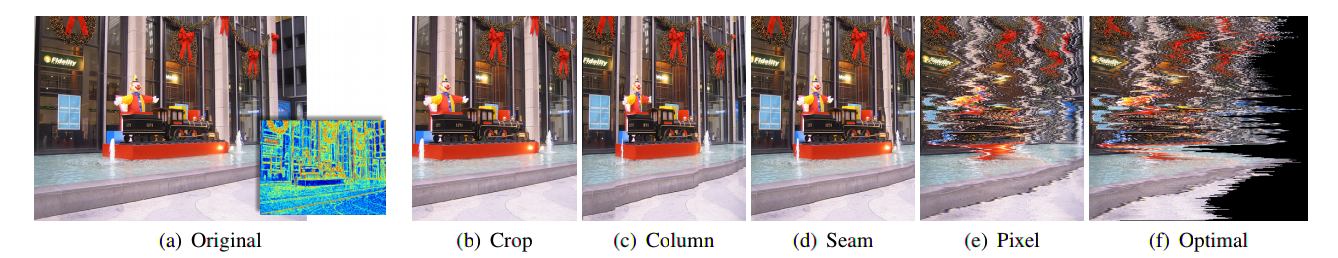
\psfig{file=ReducingStrategies.png,width =3in}
\caption{Examples}
\label{fig:singleColumnFigure}
\end{figure}

Your initial reaction might be to just remove the x number of pixels with the lowest energy but in doing so you will no longer have a rectangular image (figure 1f)\cite{Avidan:2007:SCC:1276377.1276390}. You must remove an equal number of pixels from each row (or column). However just removing the lowest energy pixel from each row over and over will leave you with a mess (figure 1e)\cite{Avidan:2007:SCC:1276377.1276390}. So the next logical step would be to just remove the lowest energy columns. However this still distorts our image and creates obvious jumps in the image, evident in the diagonal floorboard line (figure 1c)\cite{Avidan:2007:SCC:1276377.1276390}. This leads us to seams. A seam is simply a \begin{quote}a trail of pixels traversing the image from the bottom to the top, and at each step the pixel trail can veer to the right or left by at most one pixel.\cite{blogPost}\end{quote}
Let image I be a n$\times$m image and a vertical seam is: 


$s^{x}$ = \{s$_i^x$\}$_{i=1}^{n}$ = \{(x(i),i)\}$_{i=1}^n$ , s.t. $\forall$i,|x(i)-x(i-1)| $\leq$ 1 
\cite{Avidan:2007:SCC:1276377.1276390}



Meaning that the seam will start at the top of the image and traverse down to the bottom, always increasing y by 1 to include a pixel in each row. This definition also requires that the next pixel in the row above the place you currently are either is directly above you current location, one pixel to the left, or one pixel to the right. This insures that the seam stays connected. This same definition holds for horizontal seams when you swap the x’s for y’s and the n’s for m’s. Then when a seam is removed all the pixels will shift left (or up) to fill in the missing seam. 
I only briefly described which pixels constitute being called low energy. There are different energy functions that can be used to measure this. I will be describing a method that looks at the surrounding pixels to decide if different enough.  If we have a color image I with each pixel having a location in the image (x, y) and a color value (r, g, b) we can calculate the partial derivative  to find the energy. A way to approximate this value is by looking at the surrounding pixels I(x-1, y), I(x+1, y), I(x, y-1), I(x, y+1) and using those to find the partial derivatives in each direction:

|I(x+1, y) - I(x-1, y)|/2 for the x direction and |I(x, y-1) - I(x, y+1)|/2 for the y direction

\cite{Avidan:2007:SCC:1276377.1276390}

We will then sum the horizontal and vertical derivatives to get one value that we will call the energy level. 
e(I) = | ∂ /∂ x I|+| ∂/ ∂ y I|
Now that we know the energy function and what constitutes a seam we need to traverse through the image to find the lowest cost seam. We will use dynamic programming to accomplish this. In this case dynamic programming uses sub seams that we have already calculated when calculating multiple longer seams so we don’t need to calculate that sub seam multiple times.
M(i, j) = e(i, j)+ min(M(i−1, j −1),M(i−1, j),M(i−1, j +1)) 
\cite{Garey:1979}

\section{Improved Methods}
\label{sec:improvedMethods}

\section{Discussion}
\label{sec:discussion}

\section{Conclusion}
\label{sec:conclusion}


\section*{Acknowledgments}
\label{sec:acknowledgments}

This section is optional; it is a location for you
to acknowledge grants, funding, editing assistance and
what have you.

% The following two commands are all you need in the
% initial runs of your .tex file to
% produce the bibliography for the citations in your paper.
\bibliographystyle{abbrv}
% sample_paper.bib is the name of the BibTex file containing the
% bibliography entries. Note that you *don't* include the .bib ending here.
\bibliography{sample_paper}  
% You must have a proper ".bib" file
%  and remember to run:
% latex bibtex latex latex
% to resolve all references

\end{document}
